
\section{General outline on key issues}
Currently existing solutions are not robust enough to supplement current voting schemes. Most of them incur technical cost to understand crypto-currencies, are riddled with implementation issues and vulnaribilities or lack of decentralized idenitity proof [VARSHNEYA~et~al.~2015].\par
The following chapter will focus on open issues arising with blockchain based electronic voting systems.

\subsection{Blockchain identity issue}
%\begin{figure}[H]
%\centering
%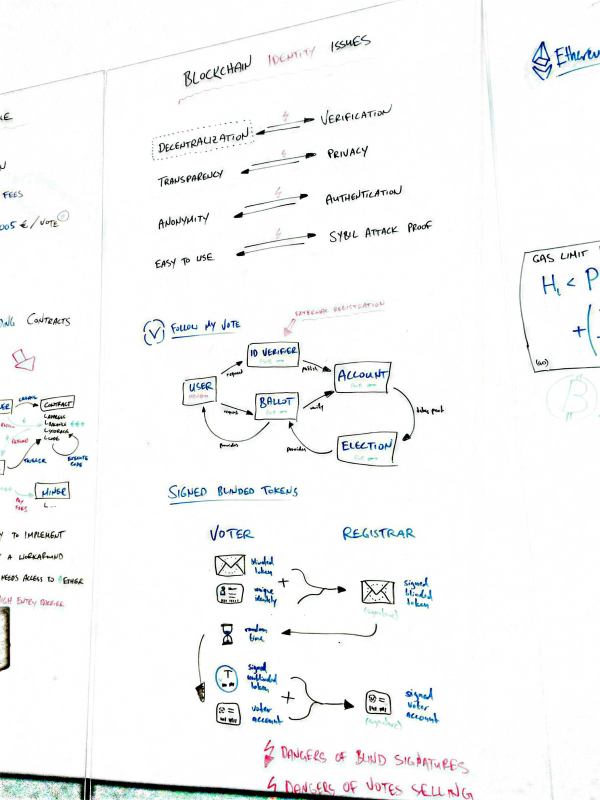
\includegraphics[draft,width=0.3\textwidth]{img/ident.png}
%\caption{ident.}
%\label{fig:ident}
%\end{figure}
% central authority against sybil attacks (trade off?)
% voter registration: signed blinded tokens [IMG: VOTER-REGISTRAR-BLINDED-TOKENS] [HOURT~2015A]

\subsection{Architecture considerations}
%\begin{figure}[H]
%\centering
%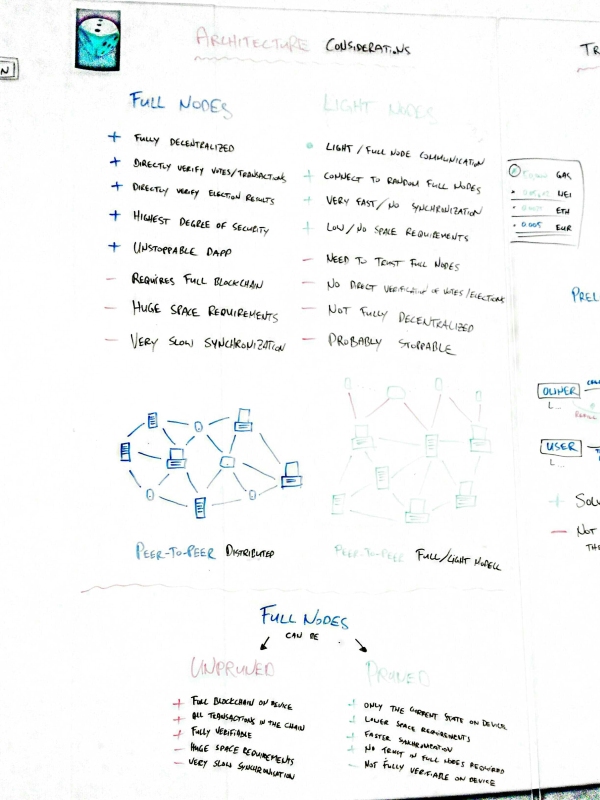
\includegraphics[draft,width=0.3\textwidth]{img/arch.png}
%\caption{arch.}
%\label{fig:arch}
%\end{figure}
For reference, the Bitcoin blockchain size is -- at the time of writing -- 63 GiB in size and growing at a rate of around 3 GiB per month. The Ethereum blockchain is 12 GiB in size and groing at a rate of 1.5 GiB per month.\par
This introduces a logistic, technical entry barrier for users of blockchain technology. The trade-off in decentralized, transparent and trustless systems is that every participant in the network stores its own copy of all available data.\par
Considering the \textit{inclusion} of every citizen in the world or a specific nation in a blockchain voting process, one has to consider the different levels of both technological understanding of each person -- regardless of age, education, social and cultural background -- and access to technology supporting distributed ledgers. Idially, any device from smartwatches, through smartphones, notebooks or workstations should be able to participate in the blockchain voting process. But storing a full copy of an underlying blockchain is not always possible.
\subsubsection{Light clients} % TODO IMAGE
A possible solution is the utilization of light nodes on small devices which connect to random full nodes on more dedicated devices. Full nodes store a copy the blockchain and are equal peers in the peer-to-peer network. They offer the highest degree of security as they can directly verify transactions, votes and election results. A network of full nodes directly connected to each other reaches the highest degree of decentralization and it's almost impossible to shut down or disrupt the network. Downsides of full nodes are the hugh space requirements for storing the full copy of the ledger and the very slow syncrhonization and verification process.\par
Introducing a light-to-full-node communication can bypass the synchronization issues and disk space requirements. This can be done by connecting to random full nodes in the network via any kind of API which offers querying the blockchain on such clients. The disadvantage of such an architecture is the need of trust towards the full nodes as they could deliver tampered data. The light clients can not directly verify transactions, votes and elections as they have no copy of the blockchain to calculate own results. This is a drawback in decentralization. By disrupting the communication between light and full clients or by setting up malicious full nodes, this system introduces serious vulnarabilies.
\subsubsection{State-trie pruning}
Ethereum adds another option to this considerations. Since Ethereum clients not only store the blockchain but the full state trie, it is possible to \textit{prune} the blockchain state history and save up to 80\% of the disk space. The default synchronization process is \textit{unpruned}. This stores the full blockchain on the device, verifies all block's proof-of-work and commits all transactions to update the state trie. This allows the client to verify any state of the blockchain in the past by querying recent states. The downside is -- as discussed earlier -- that this method has huge space requirements and a very slow syncrhonization process. An alternative is to prune the state trie. This only downloads the blockchain and verifies the proof-of-work but it does not commit all transactions included in the blocks. The whole state history is not calculated. After the blockchain was downloaded, the client requests the latest state from other nodes and saves it.\par
State-trie-pruning nodes might be the way to go as in most cases only the current state is interesting for the clients. This lowers space requirements and speeds up blockchain synchronization without introducing a gap of trust between nodes as seen with light client architectures. The only downside is the lack of the full state trie \textit{history}.
% @TODO BIGCHAIN DB

\subsection{Blockchain voting scalability}
%\begin{figure}[H]
%\centering
%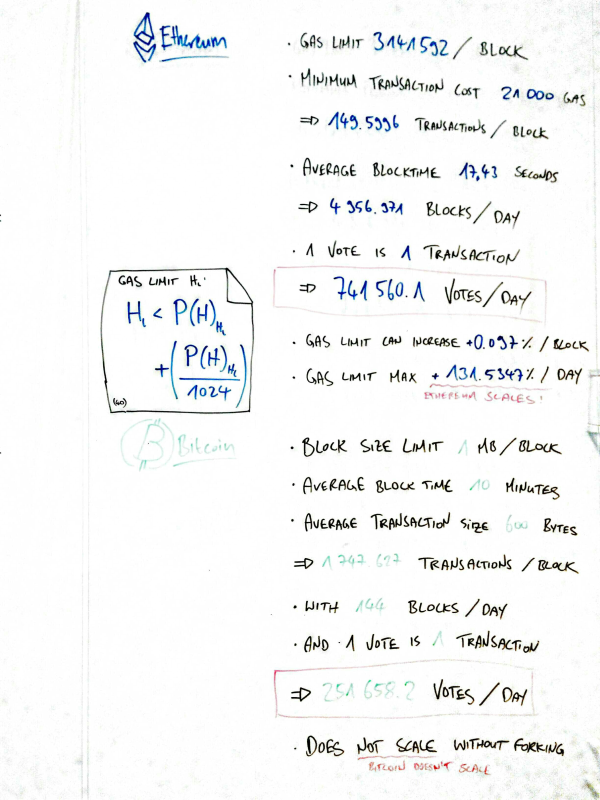
\includegraphics[draft,width=0.3\textwidth]{img/scale.png}
%\caption{scale.}
%\label{fig:scale}
%\end{figure}
Blockchain scalability is a hot debated topic right now. The Bitcoin blockchain has reached a state where almost each block in the network reached its maximum size of 1 MiB and on busy days the backlog of unconfirmed transactions piles up to several thousend transactions. The following scalability considerations will be made on a worst-case assumption which requires each vote to be a single signed transaction.
\subsubsection{Bitcoin scalability}
The Bitcoin block size limit is hardcoded at 1 MiB per block. The average block time is 10 minutes and the average transaction size to transfer funds is around 600 Bytes. This allows an average maximum of around 1748 transactions per block.
\begin{eqnarray}
& & \frac{1 \cdot 1024 \cdot 1024 B}{600 B} = 1747.62667 \frac {tx} {block}
\end{eqnarray}
With an average of 10 minutes per block there are 144 blocks per day.
\begin{eqnarray}
& & \frac{60 min \cdot 24 h}{10 \frac{min}{block}} = 144 \frac {blocks}{day}
\end{eqnarray}
With the assumption that one vote is one transaction and the blockchain is not used by anything else but voting, this allows roughly 251,659 votes per day.
\begin{eqnarray}
& & 144 \frac {blocks}{day} \cdot 1747.62667 \frac {tx} {block} = 251658.24 \frac{tx}{day}
\end{eqnarray}
Comparing that figure with numbers of registered voters in general elections around the world, one get's the idea what kind of limits this introduces. A big downside of Bitcoin is the unability to scale the number of transactions per time without introducing any network forks. Possible solutions exist but there is no consensus on which solution to use. Currently Bitcoin does \textit{not} scale.
\subsubsection{Ethereum scalability}
[SCHIENER~2015B] analyzed Ethereum blockchain voting and noticed that it would take around 40 days to hold the general elections of the United Kingdom on the Ethereum network. He gathered data from his own voting prototype which was not optimized regarding transaction size and also did not take into account that the block size is not fixed in Ethereum.\par
The Ethereum network determines fees by utilizing \textit{Gas}. Each transaction costs a certain amount of gas and each block has a block gas limit which determines the maxium of gas which can be spent each block. The current default gas limit of the Ethereum network after the Homestead release in March 2016 is 4,712,388 gas per block. The minimum cost of a transaction -- most likely just for transferring funds -- is 21,000 gas. This allows around 225 transactions per block by default.
\begin{eqnarray}
& & \frac {4712388 \frac{gas}{block}}{21000\frac{gas}{tx}} = 224.39943 \frac{tx}{block}
\end{eqnarray}
The current average block time is 15 seconds. Therefore, the network generates around 5760 blocks per day.
\begin{eqnarray}
& & \frac{60 min \cdot 24 h}{15 \frac{sec}{block}} = 5076 \frac {blocks}{day}
\end{eqnarray}
With the assumption that one vote is a transaction of minimal size and the network is not used for anything else, this allows to process 1,292,541 votes per day.
\begin{eqnarray}
& & 5076 \frac {blocks}{day} \cdot 224.39943 \frac {tx} {block} = 1292540.70857 \frac{tx}{day}
\end{eqnarray}\par
But that's only the default network capacity. Referring to the Ethereum yellow paper equations 44-46, the block gas limit scales as follows [WOOD~2014]:
\begin{eqnarray}
& & H_l < {P(H)_H}_l + \left\lfloor\frac{{P(H)_H}_l}{1024}\right\rfloor \quad \wedge \\ % 44
& & H_l > {P(H)_H}_l - \left\lfloor\frac{{P(H)_H}_l}{1024}\right\rfloor \quad \wedge \\ % 45
& & H_l \geqslant 125000 % 46
\end{eqnarray}
Simplyfied, this allows each block to grow by $1 + \frac{1}{1024}$ in terms of block gas limit. This allows a theoretic maximum increase of the block size limite by factor 142 per day.
\begin{eqnarray}
% & & \left( 4712388 \frac {gas}{block} + \frac{4712388 \frac {gas}{block}}{1024} \right) ^ {5076 \frac {blocks}{day}} = 141.82762
& & \left( 1 + \frac{1}{1024} \right) ^ {5076 \frac {blocks}{day}} = 141.82762
\end{eqnarray}
Ethereum scales by design only limited by physical boundaries like bandwith, available disk space and the central processing unit.
% [IMG: SCALABILITY-BTC-VS-ETH]

\subsection{Transaction fees issue}
%\begin{figure}[H]
%\centering
%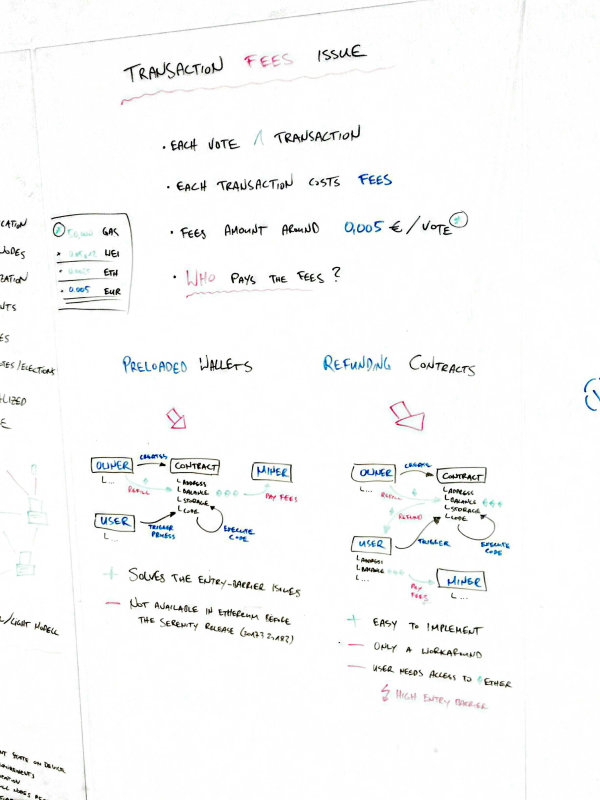
\includegraphics[draft,width=0.3\textwidth]{img/fees.png}
%\caption{fees.}
%\label{fig:fees}
%\end{figure}
Distributed ledgers are not controlled by anyone. Therefore, mechanisms have to be introduced which prevent spam or abuse of the network. Blockchain technology depends on fees which are usually paid by the signer of a transaction.\par
This introduces issues regarding several applications which operate on top of blockchains. Even though the fees are very low -- sometimes just a fraction of a cent -- they introduce an entry barrier for instance to interact with smart contracts or to vote on a blockchain.\par
Updating the records of the public ledger always costs fees. A fee worth less than a cent makes network attacks expensive but also requires every participant of the network to have access to the underlying currency. Decentralized applications must offer free transaction models to compete with centralized alternatives. Daniel Larimer of the Bitshares project adds, \enquote{it doesn't matter how good the service is, people expect certain things to be free} [LARIMER~2016].\par
Dominik Schiener calculated the average fees based on his proof-of-concept implementation would cost around 0.0091875 USD per vote [SCHIENER~2015B]. He further concluded, voting on blockchain is far cheaper compared to the costs of the general elections in the United Kingdom. However, any fee -- as low as it could ever be -- will just prevent a majority of potential users to use such applications.\par
A practical solution is still outstanding. Five approaches should be discussed for integration into future blockchain projects.
\subsubsection{Fractional reserve}
Larimer further suggests a dynamic fractional reserve which eliminates fees and introduces a model based on available \textit{bandwith} to write on the blockchain. The bandwidth is determined by how much stake (e.g., coins, gas) a participant in the network has [LARIMER~2016]. This is certainly a promising appraoch, but is still not free as users would have to hold any form of currency. This does not solve the underlying issue because it does not remove the initial entry barrier.
\subsubsection{Transaction server}
Schiener introduces a central polling server, which signes the transactions of the voters and pays the transaction fees [SCHIENER~2015A]. The fees are prefilled by the creator of the election. But this, however, introduces other issues, as discussed in section \ref{sec:pubv}.
\subsubsection{Refunding contracts}
Another approach could involve smart contracts refunding senders of transactions addressed at the contract. The creator of a poll fills the balance of the contract account and the user gets a refund after triggering the code execution on the contract based on his spent fees. This solution should be among the most easy ones to implement, however, it also does not remove the need to hold any unit of a crypto-currency. In addition, this might allow malicious parties to repeatedly call the contract to deplete its funds. % opens a door for spam or abuse of the network, as the user never faces any costs except the initial gas required to invoke the contract.
\subsubsection{Forwarding contracts}

%contract Gracious {
%  function runMe() {
%    this.realWork.gas(1000000)();
%  }
%}

\subsubsection{Contract pays}
The current model of most blockchain environments implements the earlier described \enquote*{sender pays} method where the signer of a transaction has to cover the fees. Recent advances in smart contract technology plan to implement new models.\par
Rootstock, which builds a smart contract platform on top of the Bitcoin platform, introduces an \enquote*{author pays}.
%One elegant blockchain implementation would offer the
%for some dapps, “contract pays” is a better model than “sender pays” as senders may not have any ether; now, individual dapps can implement such models, and if they are written in a way that miners can statically analyze and determine that they actually will get paid, then they can immediately accept them []

\subsection{Decentralized deadline consensus problem}
% decentralized deadline consensus problem: how to determine whether a message was sent before a certain deadline in a private, trustless, distributed system? [BORGSTRUP~2014]
% solution: dec cons deadl protocol [BORGSTRUP~2014]
% uses bitcoin nodes to create timestamps, costs fees [BORGSTRUP~2014]
% message interpretation layer on top of bitcoin timestamping, which handles msgs as votes [BORGSTRUP~2014]

\subsection{Voting coercion in distributed systems}
% possibility of revoting against coercion [BORGSTRUP~2014]

% steps of voting are transactions on the blockchain [HOURT~2015B]
% id verification -> transaction [HOURT~2015B]
% each id voted at most once [HOURT~2015B]
% broadcast new transaction for each decision change

% revoting: chaining votes with previous trx hashes [BORGSTRUP~2014]

\subsection{Power distribution with proof-of-work}
% pow, pos lottery
% a+b > 51%
% disruption of processing
% possible solution federated transaction consensus
% equal distribution of power, control
